Throughout project development, several datasets from various sources have been used to fulfil Magpie's project goal. Below is an overview of Magpie's data sources:
\begin{figure}[h!]
    \centering
    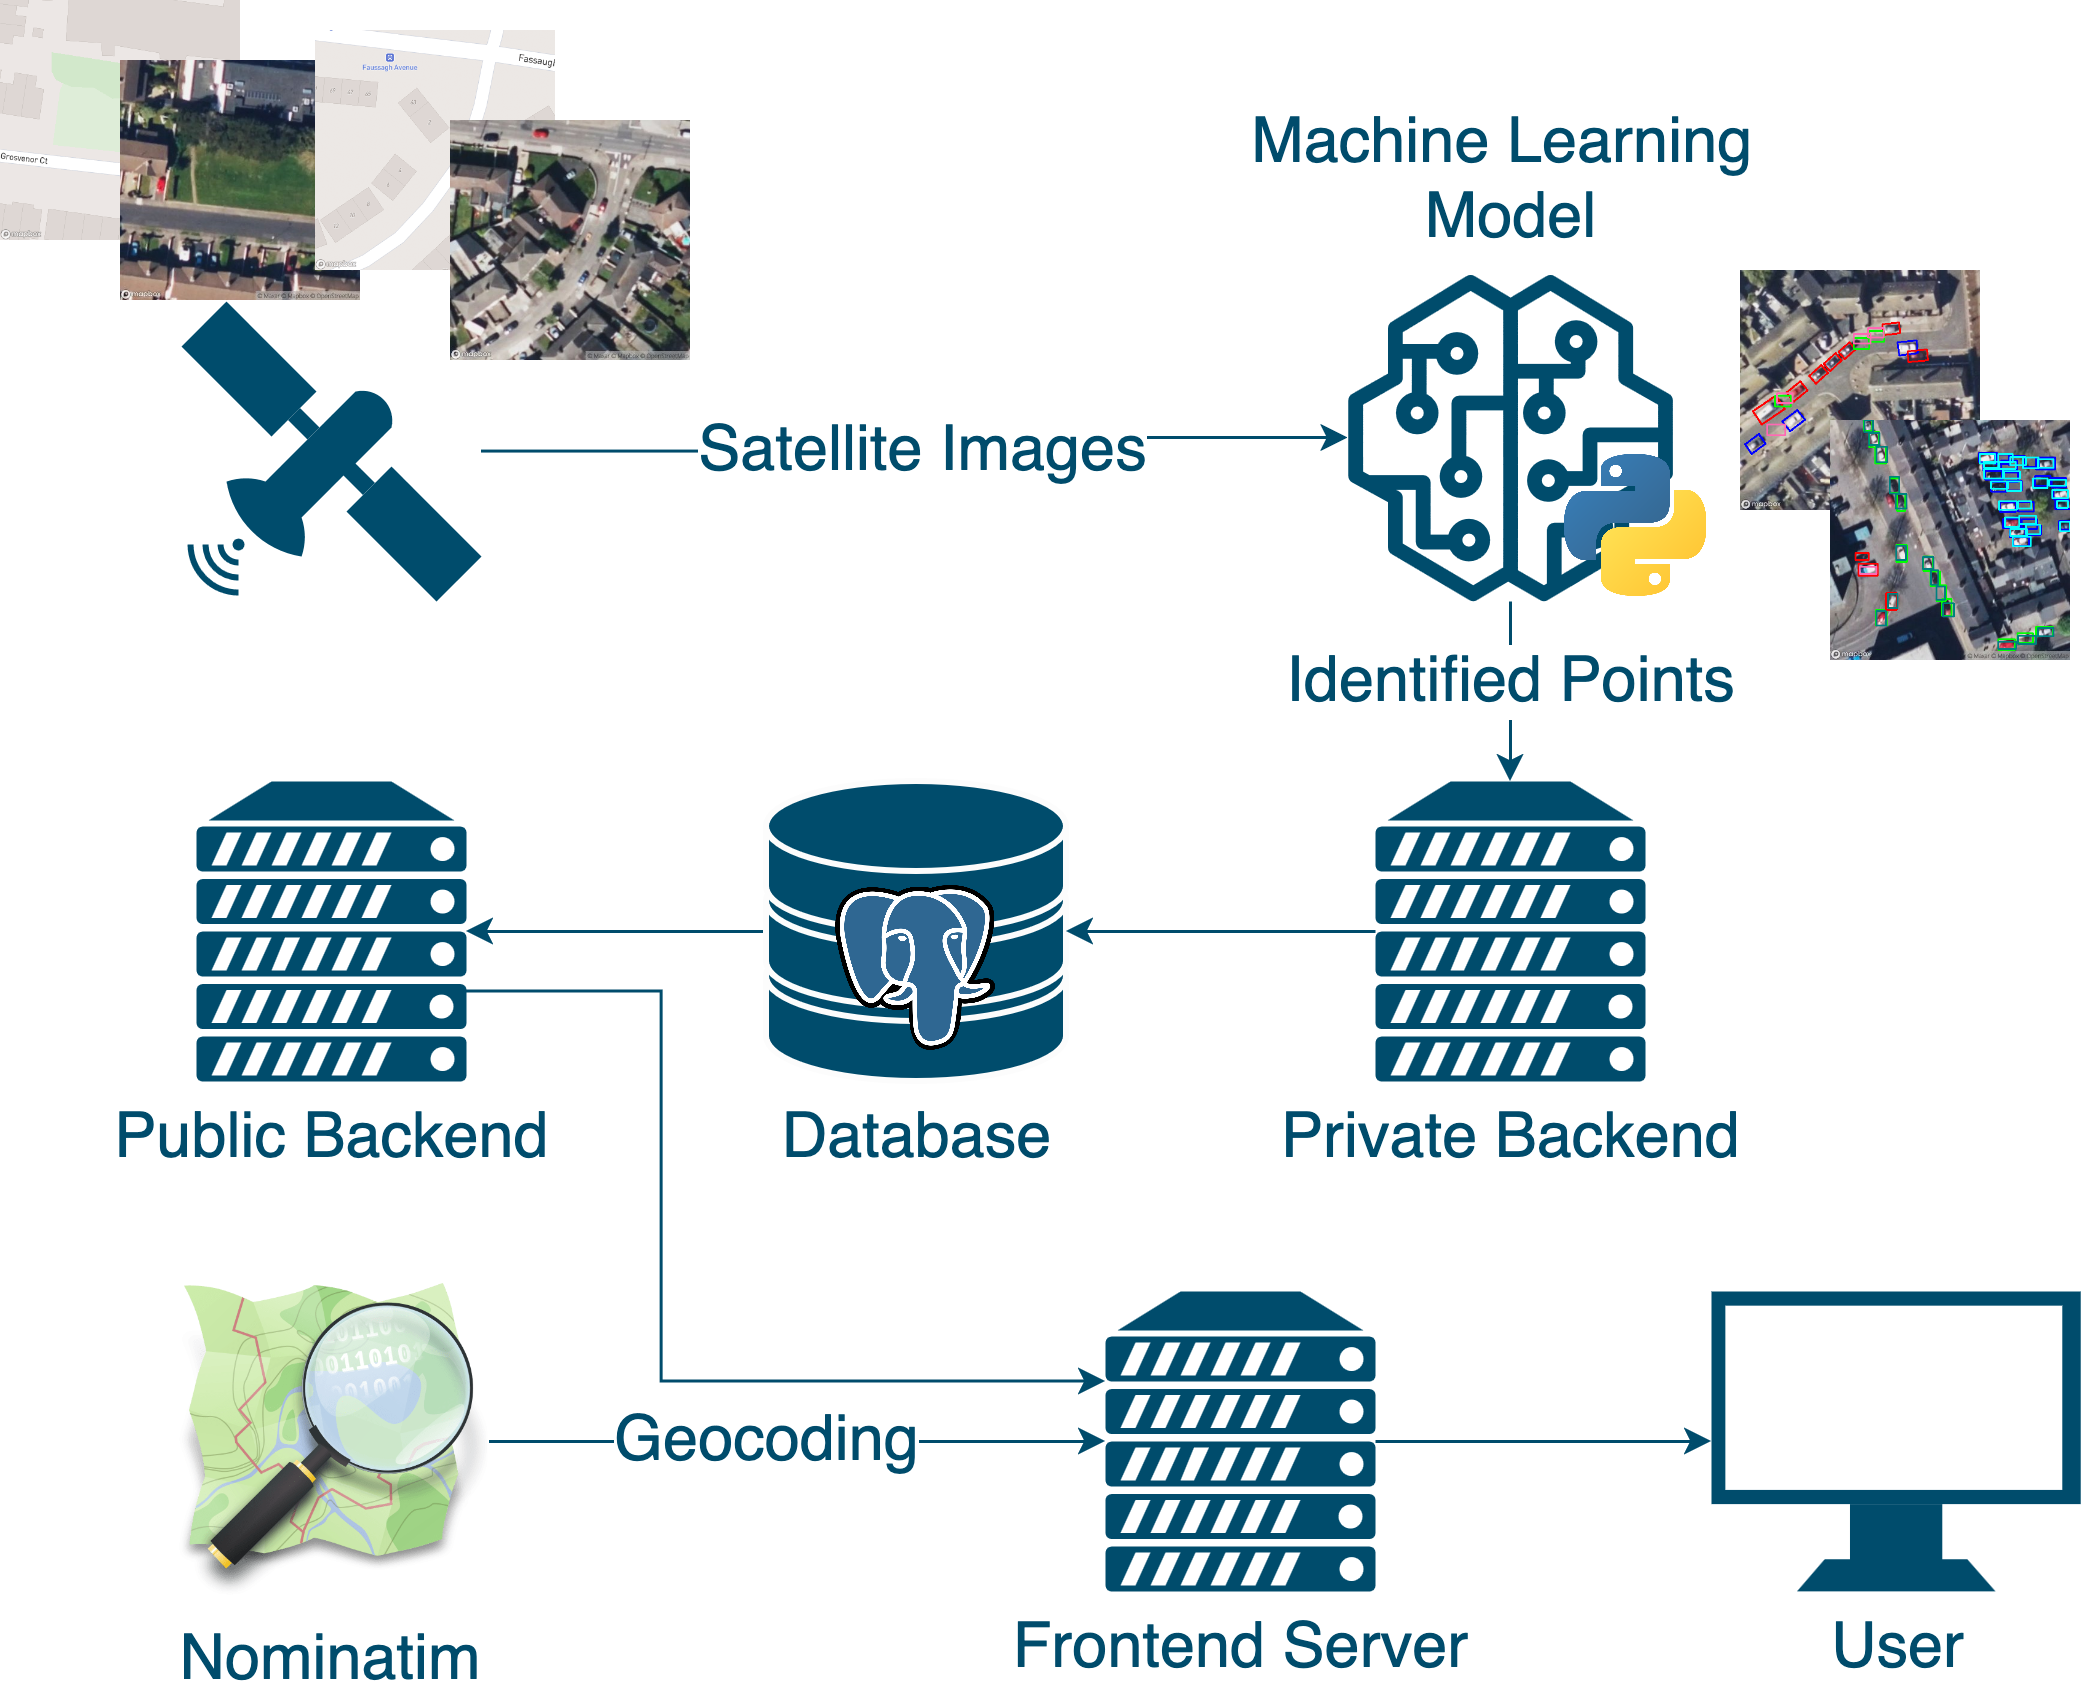
\includegraphics[width=0.85\textwidth]{images/magpie-data-stack.png}
    \caption{Magpie Data Stack}
\end{figure}\\

\subsubsection{for the Machine Learning models}
\textbf{Car detection model}
Using the MapBox API, 250 images were downloaded using CSV data from the following sources:
\begin{itemize}
    \item Data.gov.ie : Online portal containing thousands of publicly available datasets about Ireland
    \item Smart Dublin: Founded by Dublin local authorities, their goal is to look for innovative technological solutions for local environmental, social, mobility, government and living issues. They also have hundreds of publicly available datasets
    \item Kaggle: a data science and machine learning platform part of Google Cloud where competitions are hosted, in addition to thousands of publicly available datasets
\end{itemize}
These CSV files contained information on the location of certain facilities such as rentals, coach parking, public parks. This location was latitude and longitude which we needed to input into the script to download images, as well as the street name of that location which was used to name the downloaded image.
\begin{listing}[h!]
    \centering
    \begin{minted}{python3}
        # CSV file containing location information
        df = pd.read_csv("2020-coach-parking-dcc-1.csv")
        location_data = df.to_dict('records')

        # function to download image using location information from CSV dataset
        def get_images(name, latitude, longitude):
            url = f'https://api.mapbox.com/styles/v1/mapbox/satellite-v9/static/{longitude},{latitude},18,0,0/400x400?access_token=pk.eyJ1Ijoia2F1c3R1Ymh0cml2ZWRpIiwiYSI6ImNtMWo2NndsbzB4N3EycHM1aGF2cDd5NzkifQ.4aegzX6Kfy3zW8pHkLWU7Q'
            response = requests.get(url)
            print(response)
            if response.status_code == 200:
                img = Image.open(BytesIO(response.content))
                if not os.path.exists('output'):
                    os.makedirs('output')

                output_folder = 'output'
                output_path = os.path.join(output_folder, f'{name}_coach_parking.png')
                img.save(output_path)
                print(f"Image saved to {output_path}")

        # function to extract location \& name location from CSV dataset
        for place in location_data:
        name = place["Street Name"]
        if ("/" in name):
            name = name.replace("/", "-")
        latitude = place["Latitude"]
        longitude = place["Longitude"]
        get_images(name, latitude, longitude)
    \end{minted}
\end{listing}\\
Following successful model training and tuning, a further 19,536 satellite images were downloaded spanning Dublin City area illustrated in the figure below.
\begin{figure}[h!]
    \centering
    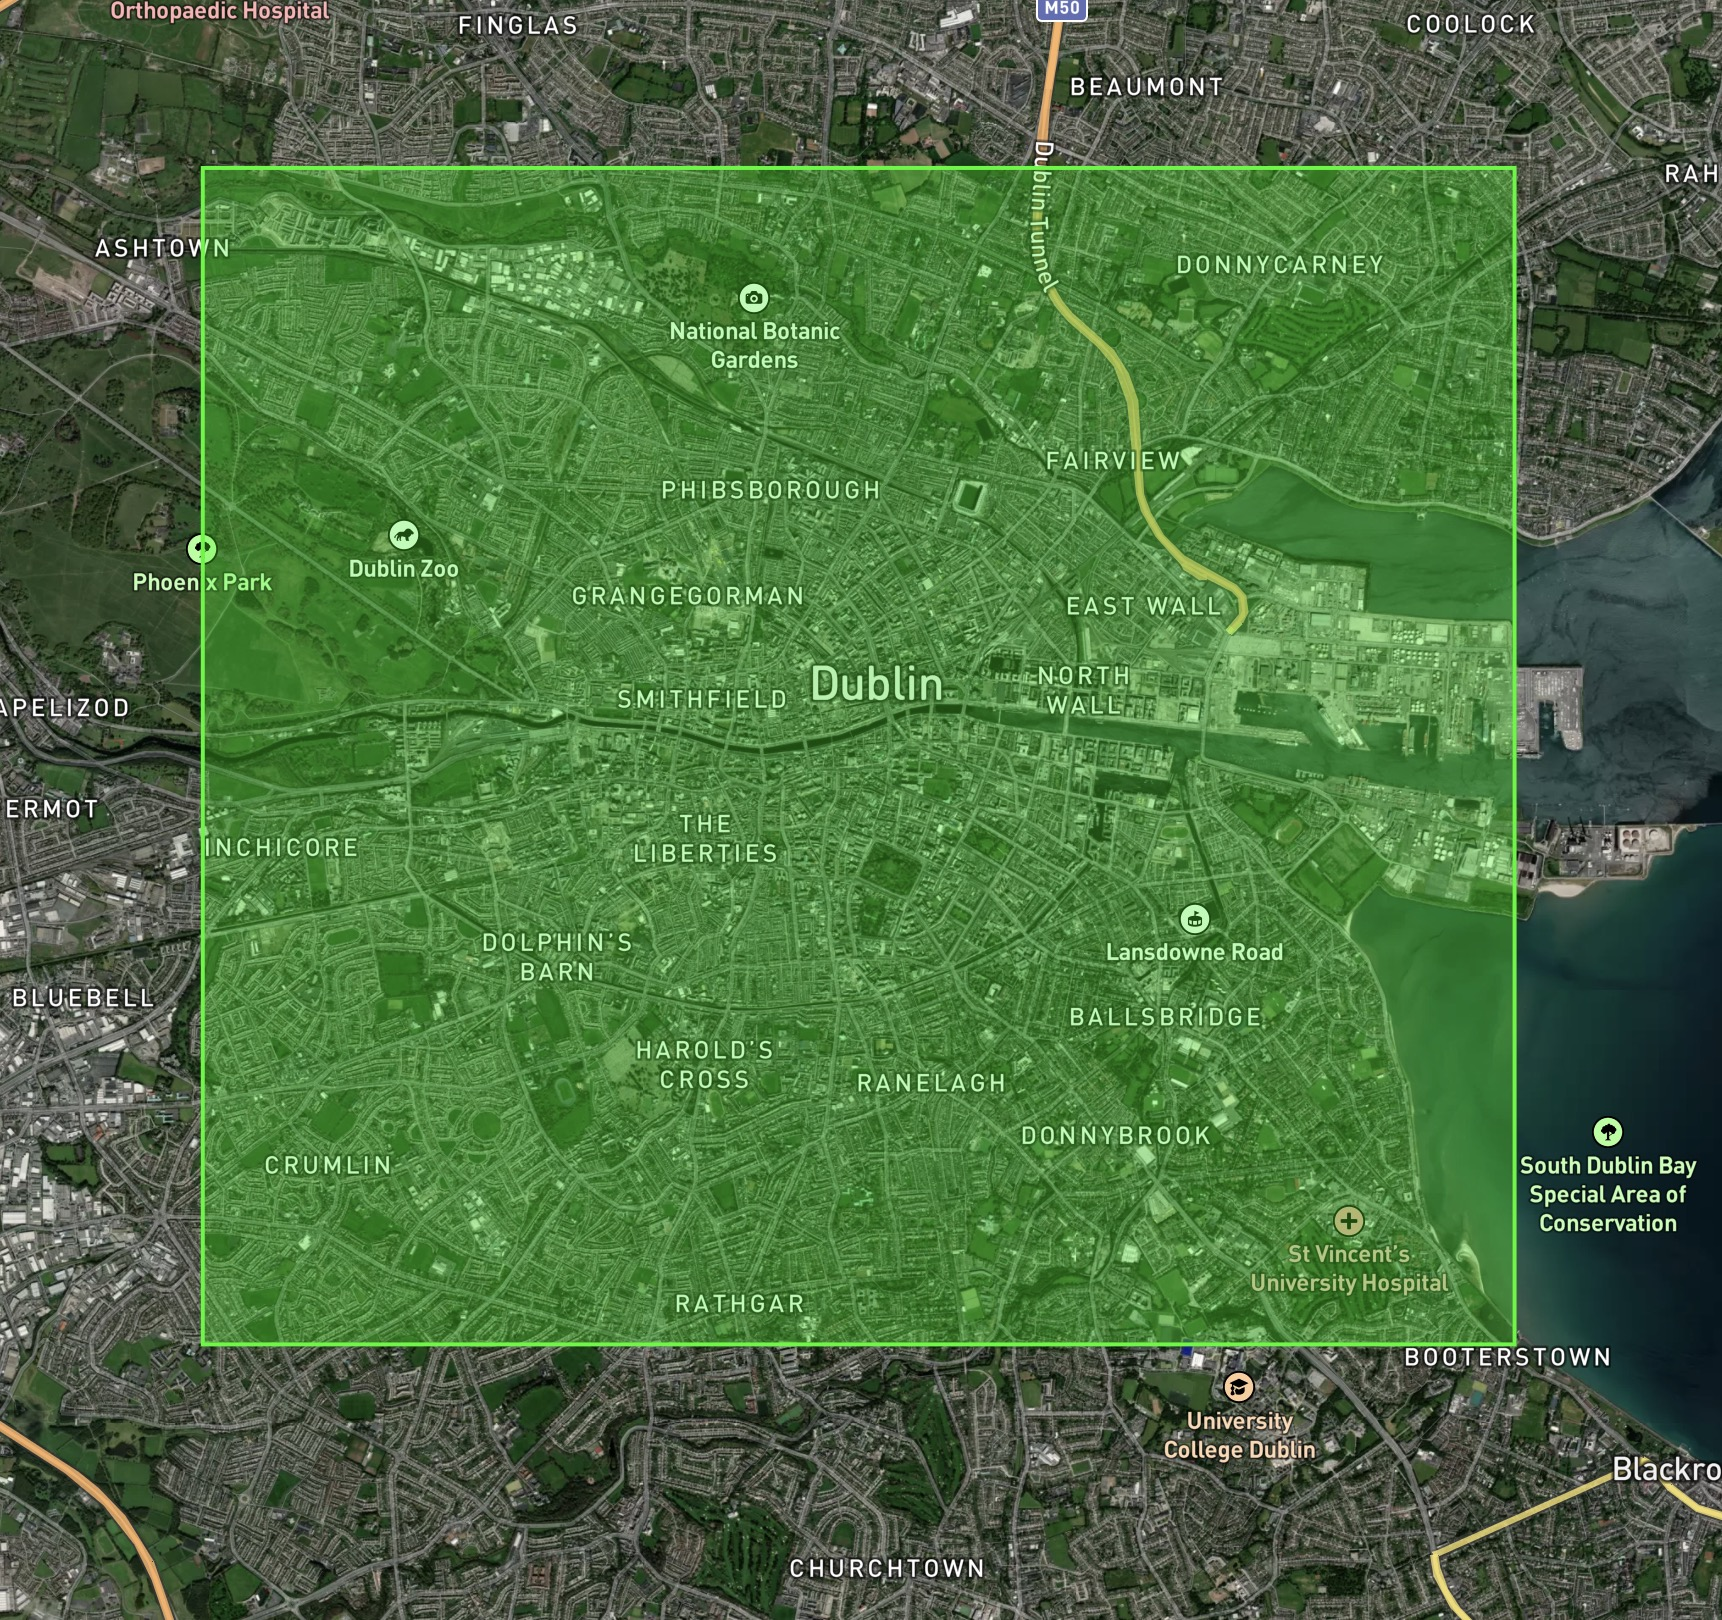
\includegraphics[width=0.85\textwidth]{images/dublin-img-area.jpg}
    \caption{Dublin Area Delimitation for Parking data}
\end{figure}\\

The machine learning model was then applied to those images to detect the cars.\\

\textbf{Parking detection model}
An additional 19,536 map-view images corresponding to the satellite images used for car detection were downloaded using the MapBox API to create the custom mask used for detecting parked cars.


\subsubsection{for the Amenity data}
CSV files were collected from multiple sources mentioned above, notable Data.gov.ie and Smart Dublin. Below is a list relative to each amenity currently present on Magpie:
\begin{itemize}
    \item Parking meter = Data.gov.ie
    \item Bike stand = Data.gov.ie
    \item Public Wifi = Smart Dublin
    \item Library = Smart Dublin
    \item Multi-storey Car park = Data.gov.ie
    \item Drinking water fountain = Data.gov.ie
    \item Public toilet = Data.gov.ie
    \item Bike sharing station = Data.gov.ie
    \item Car parking = Novel ML technique
    \item Accessible parking = Data.gov.ie
    \item Public bins = Smart Dublin
    \item Coach parking = Data.gov.ie
\end{itemize}